\section{Ejercicio N03 - Gestión de proyectos } 

Este esquema E / R simplificado muestra un caso gestión del proyecto.
El proyecto para un cliente se divide en varios paquetes de trabajo y siempre una persona es responsable de completar la
tarea. Se cuida en un lugar determinado.
La dimensión de tiempo consiste de día, mes y año.


	\begin{center}
	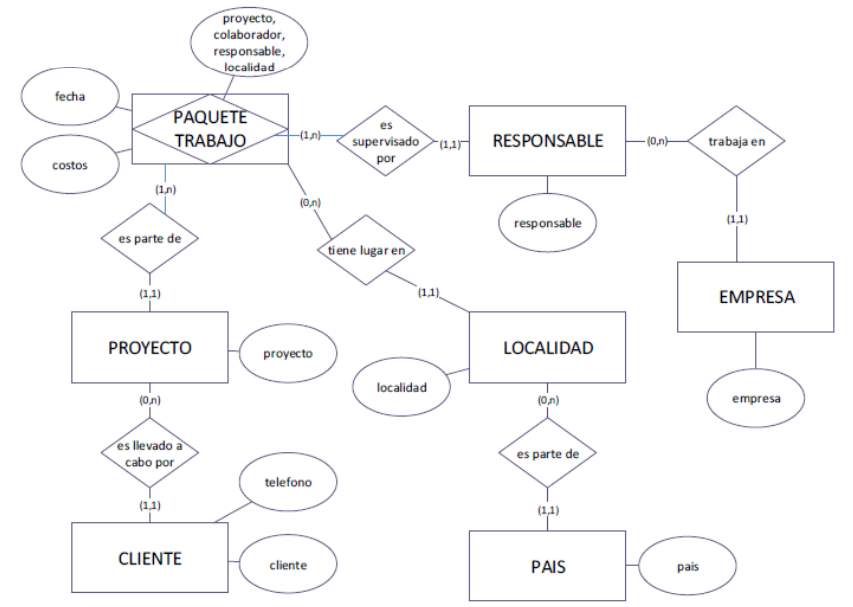
\includegraphics[width=17cm]{./Imagenes/ejercicio3}
	\end{center}	

Por favor identifique el hecho de interés y construya el Modelo Dimensional. Incluya un atributo de hecho adicional que
cuente la cantidad de paquetes de trabajo. Asimismo, realice el diagrama físico.
\\

\begin{itemize}
    \item \textbf{Modelo Dimensional}
\\
El diseñador de software ERWIN permite que se pueda crear y modificar diagramas con facilidad, mejorando la calidad de los diseños de software. El Modelo Dimensional es el resultado directo de la llegada del diseño de flujo de datos y análisis estructural.

	\begin{center}
	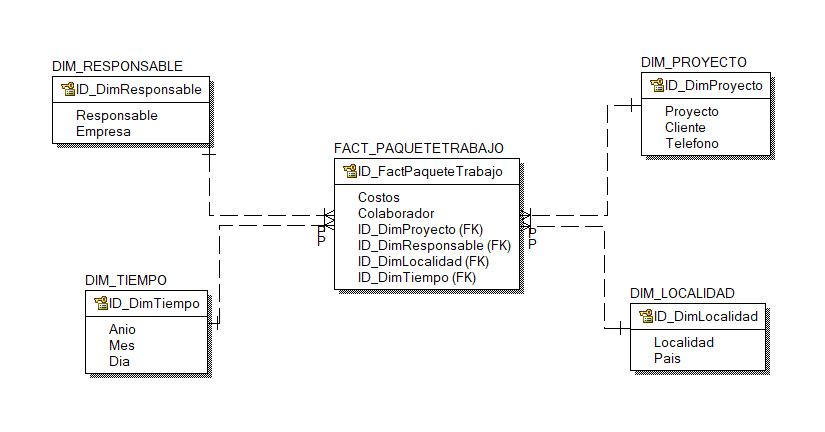
\includegraphics[width=17cm]{./Imagenes/Ejercicio3Logico}
	\end{center}	

    \item \textbf{Modelo Fisico}

Es posible crear y modificar bases de datos de forma visual a través de los diagramas de bases de Datos. Estos diagramas fisicos proporcionan una visión gráfica de las tablas en la base de datos incluyendo sus columnas, el modelo E/R y el diagrama fisico de estructura de datos en SQL Server.

	\begin{center}
	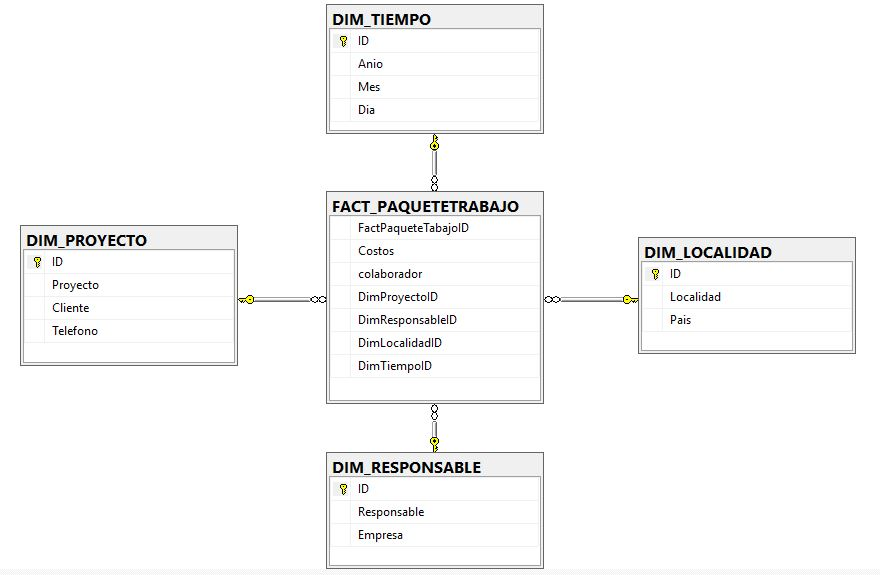
\includegraphics[width=17cm]{./Imagenes/Ejercicio3Fisico}
	\end{center}	

    \item \textbf{Código del Modelo Fisico}

	\begin{center}
	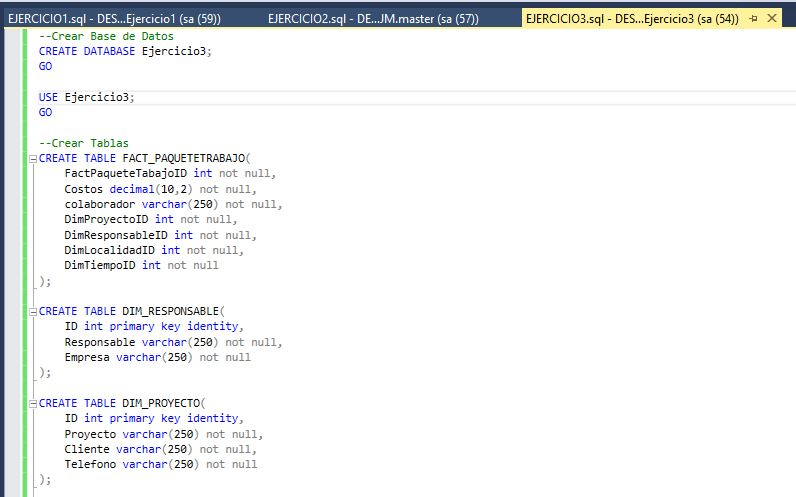
\includegraphics[width=17cm]{./Imagenes/Ejercicio3Fisico1}
	\end{center}	

	\begin{center}
	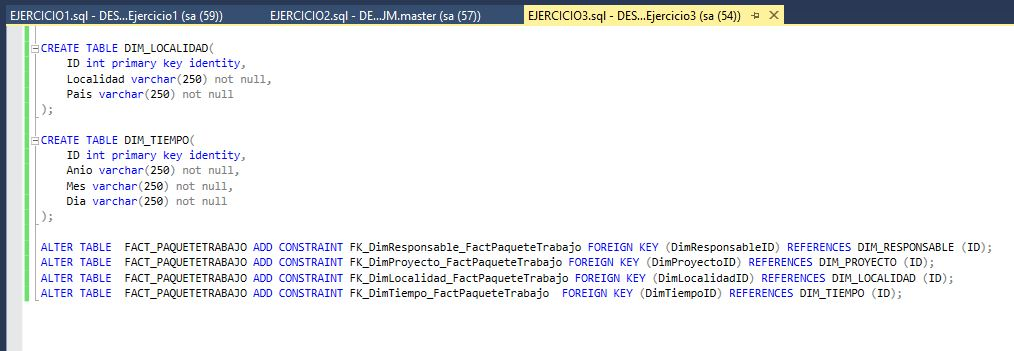
\includegraphics[width=17cm]{./Imagenes/Ejercicio3Fisico2}
	\end{center}	
\end{itemize}